\documentclass[UTF8,11pt,a4paper]{ctexart}

\usepackage[a4paper,margin=2.4cm]{geometry}
\usepackage{amsmath,amssymb,bm}
\usepackage{booktabs}
\usepackage{graphicx}
\usepackage{float}
\usepackage{subcaption}
\usepackage{array}
\usepackage{longtable}
\usepackage{multirow}
\usepackage{xcolor}
\usepackage{hyperref}
\usepackage{enumitem}
\usepackage{siunitx}
\usepackage{fancyhdr}

\graphicspath{{figures/}}
\hypersetup{
  colorlinks=true,
  linkcolor=blue!55!black,
  citecolor=blue!55!black,
  urlcolor=blue!55!black
}
\setlength{\parindent}{2em}
\setlength{\parskip}{0.25em}
\setlist{nosep}

\pagestyle{fancy}
\fancyhf{}
\fancyhead[L]{神经网络与深度学习 Project 2}
\fancyhead[R]{CIFAR-10 与 Batch Normalization}
\fancyfoot[C]{\thepage}

\newcommand{\todo}[1]{\textcolor{red}{\textbf{[请填写：#1]}}}
\newcommand{\code}[1]{\texttt{#1}}

\title{\textbf{神经网络与深度学习 Project 2}\\
       CIFAR-10 图像分类与 Batch Normalization 优化分析}
\author{
  姓名：\todo{姓名}\qquad
  学号：\todo{学号}
}
\date{2026 年 6 月}

\begin{document}

\maketitle

\begin{abstract}
本文围绕 CIFAR-10 图像分类与 Batch Normalization（BN）优化机制完成两组实验。
任务一设计了一个包含二维卷积、池化、激活函数、全连接层、BatchNorm 和
Dropout 的可配置卷积神经网络，并分别比较通道数、激活函数、损失函数、
正则化方法和优化器。最佳模型采用通道数 $(64,128,256)$、ReLU、BatchNorm、
Dropout、交叉熵损失以及带动量的 SGD，在完整训练集上取得
$92.06\%$ 测试准确率和 $7.94\%$ 测试错误率。

任务二使用适配 CIFAR-10 的 VGG-A，在完整的 45,000 张训练集上公平比较
有无 BN 的训练过程。加入 BN 后，测试准确率由 $75.88\%$ 提高到 $82.50\%$，
同时显著加快收敛。进一步使用四个学习率分析跨学习率的 loss 变化范围和梯度
行为。结果表明，BN 降低了训练初期的极端不稳定性，并在大部分训练阶段取得
更低的平均 loss；但简化的连续梯度方向与局部变化指标没有显示出改善。
\end{abstract}

\noindent\textbf{代码链接：}\todo{GitHub 仓库 URL}\\
\textbf{数据集链接：}\url{https://www.cs.toronto.edu/~kriz/cifar.html}\\
\textbf{模型权重链接：}\todo{网盘或 Release URL}

\tableofcontents
\newpage

\section{实验目标}

本项目包含两个目标：
\begin{enumerate}
  \item 在 CIFAR-10 上设计并优化卷积神经网络，比较不同结构和训练策略，
        报告最佳测试结果，并通过可视化解释模型行为。
  \item 比较 VGG-A 有无 Batch Normalization 时的训练特征，并从 loss
        landscape、梯度可预测性和梯度局部变化等角度研究 BN 对优化的影响。
\end{enumerate}

\section{数据集与实验环境}

\subsection{CIFAR-10}

CIFAR-10 包含 60,000 张 $32\times32$ RGB 图像，共 10 个类别，每类
6,000 张。其中标准训练集包含 50,000 张，测试集包含 10,000 张
\cite{cifar10}。本文从标准训练集中固定划出 5,000 张作为验证集。

\subsection{运行环境}

\begin{table}[H]
  \centering
  \caption{主要实验环境}
  \begin{tabular}{ll}
    \toprule
    项目 & 配置 \\
    \midrule
    GPU & NVIDIA GeForce RTX 4060 Laptop GPU \\
    Python & 3.12.10 \\
    PyTorch & 2.9.1 + CUDA 12.6 \\
    torchvision & 0.24.1 + CUDA 12.6 \\
    随机种子 & 任务一为 42，任务二为 2020 \\
    \bottomrule
  \end{tabular}
\end{table}

\section{任务一：CIFAR-10 分类网络}

\subsection{模型结构}

本文设计的 ConfigurableCNN 由三个卷积阶段组成。每个阶段包含两层
$3\times3$ 二维卷积、可选 BatchNorm、激活函数和 $2\times2$ 最大池化。
最后使用全局平均池化、Dropout 和全连接层输出 10 类 logits。

\begin{table}[H]
  \centering
  \caption{最佳任务一模型结构}
  \begin{tabular}{clc}
    \toprule
    阶段 & 操作 & 输出通道/尺寸 \\
    \midrule
    输入 & CIFAR-10 RGB 图像 & $3\times32\times32$ \\
    Stage 1 & $(\mathrm{Conv}+\mathrm{BN}+\mathrm{ReLU})\times2$，MaxPool
            & $64\times16\times16$ \\
    Stage 2 & $(\mathrm{Conv}+\mathrm{BN}+\mathrm{ReLU})\times2$，MaxPool
            & $128\times8\times8$ \\
    Stage 3 & $(\mathrm{Conv}+\mathrm{BN}+\mathrm{ReLU})\times2$，MaxPool
            & $256\times4\times4$ \\
    分类器 & AdaptiveAvgPool，Dropout(0.3)，Linear & 10 \\
    \bottomrule
  \end{tabular}
\end{table}

该网络包含全连接层、二维卷积层、二维池化层和激活函数，满足项目的四项基础
结构要求；同时包含 BatchNorm 和 Dropout，满足高级组件要求。最佳配置共有
1,148,874 个可训练参数。

\subsection{数据预处理与训练设置}

任务一使用 45,000 张训练图像、5,000 张验证图像和全部 10,000 张测试图像。
训练阶段使用随机裁剪（padding 为 4）和随机水平翻转，随后按 CIFAR-10
通道均值和标准差归一化；验证集和测试集仅归一化。

最佳模型使用交叉熵损失、SGD 优化器、初始学习率 0.1、momentum 0.9、
weight decay $5\times10^{-4}$、batch size 128 和 cosine 学习率调度，
共训练 50 epoch。模型选择仅依据验证集准确率，最后加载最佳 checkpoint
在测试集上评估。

\subsection{消融实验}

为覆盖项目要求，分别研究以下因素：
\begin{itemize}
  \item 通道数：$(32,64,128)$ 与 $(64,128,256)$；
  \item 激活函数：ReLU 与 GELU；
  \item 损失函数：交叉熵、Focal Loss 和 label smoothing；
  \item 正则化：比较有无 Dropout 和 weight decay；
  \item 优化器：Adam 与带 momentum 的 SGD。
\end{itemize}

\begin{table}[H]
  \centering
  \caption{任务一实验结果。除特别注明外，均使用通道数
  $(64,128,256)$、BatchNorm 和 Dropout。}
  \resizebox{\textwidth}{!}{
  \begin{tabular}{lccccccc}
    \toprule
    实验 & 主要变化 & 参数量 & 最佳验证准确率 & 测试准确率 & 测试错误率 & 时间/s \\
    \midrule
    Baseline & Adam + ReLU + CE & 1,148,874 & 91.18\% & 90.25\% & 9.75\% & 191.05 \\
    Small & 通道 $(32,64,128)$ & 288,746 & 88.34\% & 87.91\% & 12.09\% & 177.09 \\
    GELU & ReLU 改为 GELU & 1,148,874 & 91.46\% & 90.67\% & 9.33\% & 164.95 \\
    Focal & Focal Loss & 1,148,874 & 90.50\% & 89.95\% & 10.05\% & 158.17 \\
    Label smoothing & smoothing $=0.1$ & 1,148,874 & 91.52\% & 90.75\% & 9.25\% & 169.31 \\
    无正则化 & Dropout$=0$，weight decay$=0$ & 1,148,874 & 90.36\% & 89.92\% & 10.08\% & 167.32 \\
    \textbf{SGD} & \textbf{SGD + momentum} & \textbf{1,148,874}
        & \textbf{92.68\%} & \textbf{92.06\%} & \textbf{7.94\%} & \textbf{296.66} \\
    \bottomrule
  \end{tabular}}
\end{table}

\subsection{结果分析}

扩大通道数使测试准确率提高 2.34 个百分点，但参数量约增至四倍，说明模型容量
对 CIFAR-10 性能有明显影响。GELU 和 label smoothing 均带来小幅提升；
Focal Loss 未改善结果，这可能是因为 CIFAR-10 各类别基本均衡，而 Focal Loss
主要针对大量易样本或类别不均衡问题。移除 Dropout 和 weight decay 后准确率
下降，说明正则化有助于泛化。SGD 最终比 Adam 高 1.81 个百分点，虽然训练时间
更长，但获得了最佳验证和测试性能。

\subsection{最佳模型及可视化}

最佳模型出现在第 47 epoch，验证准确率为 $92.68\%$，测试准确率为
$92.06\%$，对应测试错误率为 $7.94\%$。

\begin{figure}[H]
  \centering
  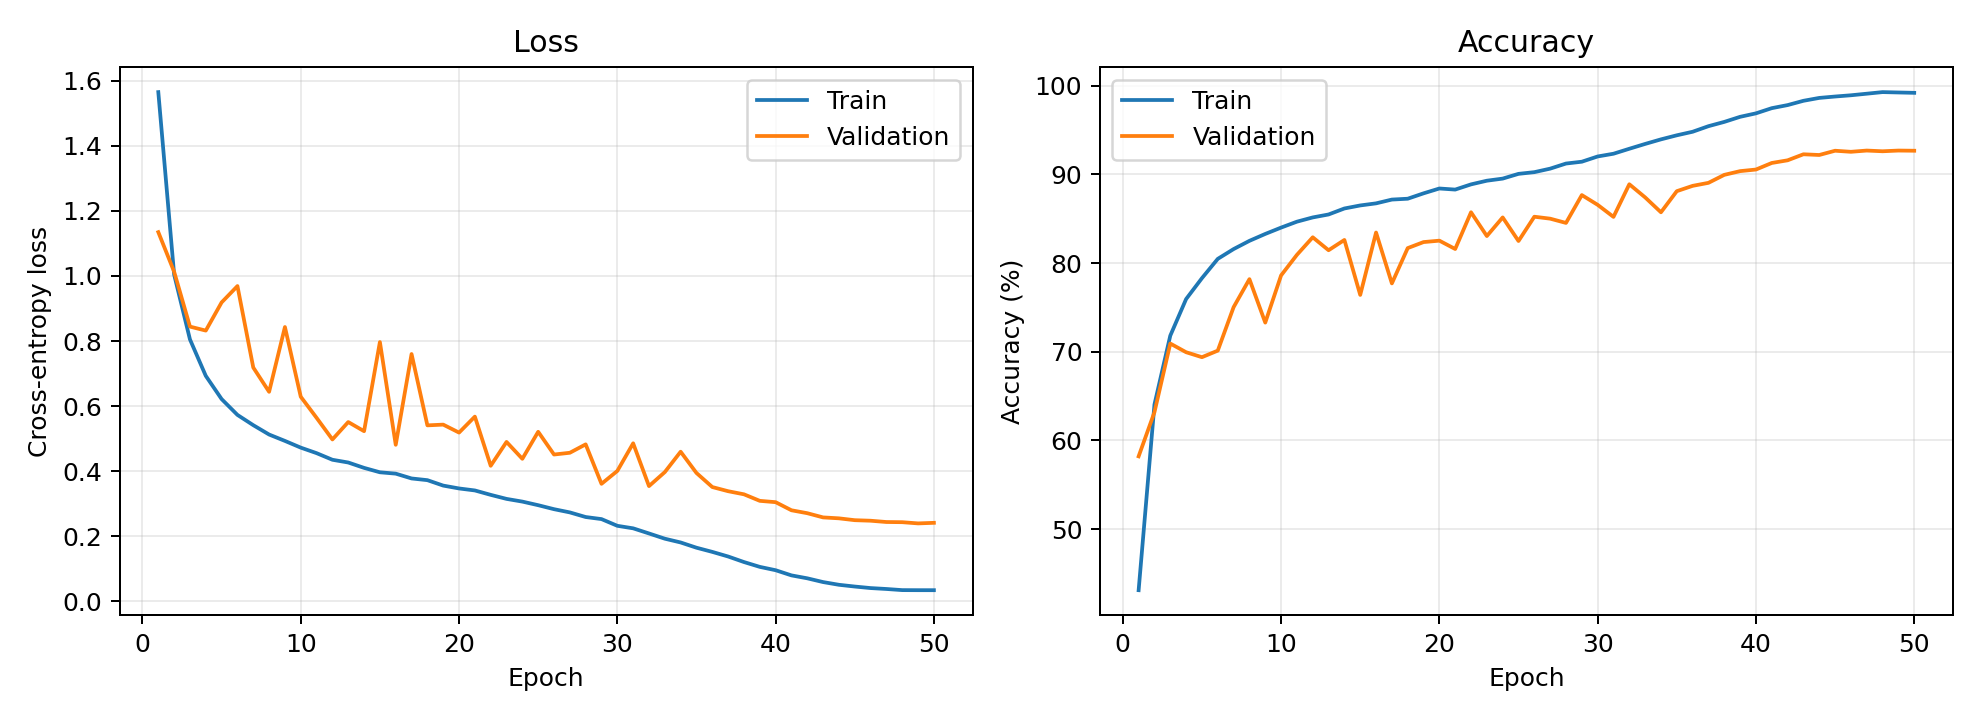
\includegraphics[width=0.95\textwidth]{task1_training_curves.png}
  \caption{最佳任务一模型的训练与验证曲线。训练准确率最终超过 $99\%$，
  验证准确率趋于稳定，说明模型已经基本收敛，同时仍存在一定泛化差距。}
\end{figure}

\begin{figure}[H]
  \centering
  \begin{subfigure}{0.49\textwidth}
    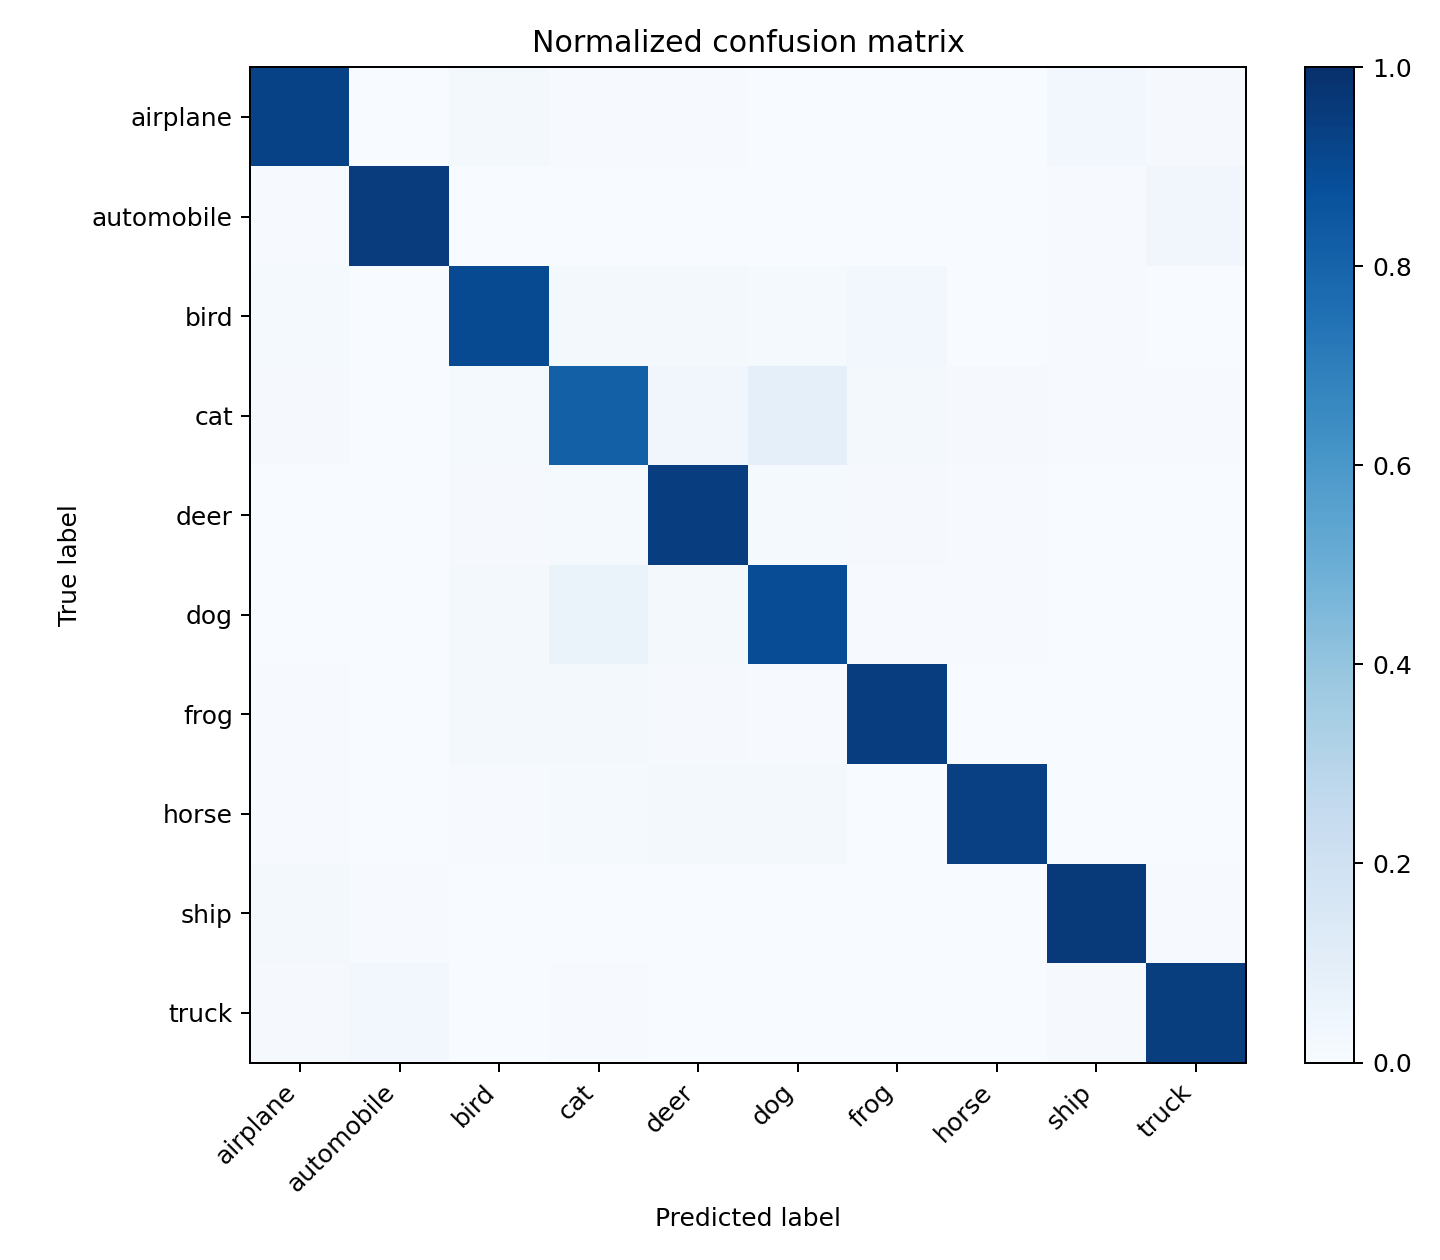
\includegraphics[width=\linewidth]{task1_confusion_matrix.png}
    \caption{归一化混淆矩阵}
  \end{subfigure}
  \hfill
  \begin{subfigure}{0.49\textwidth}
    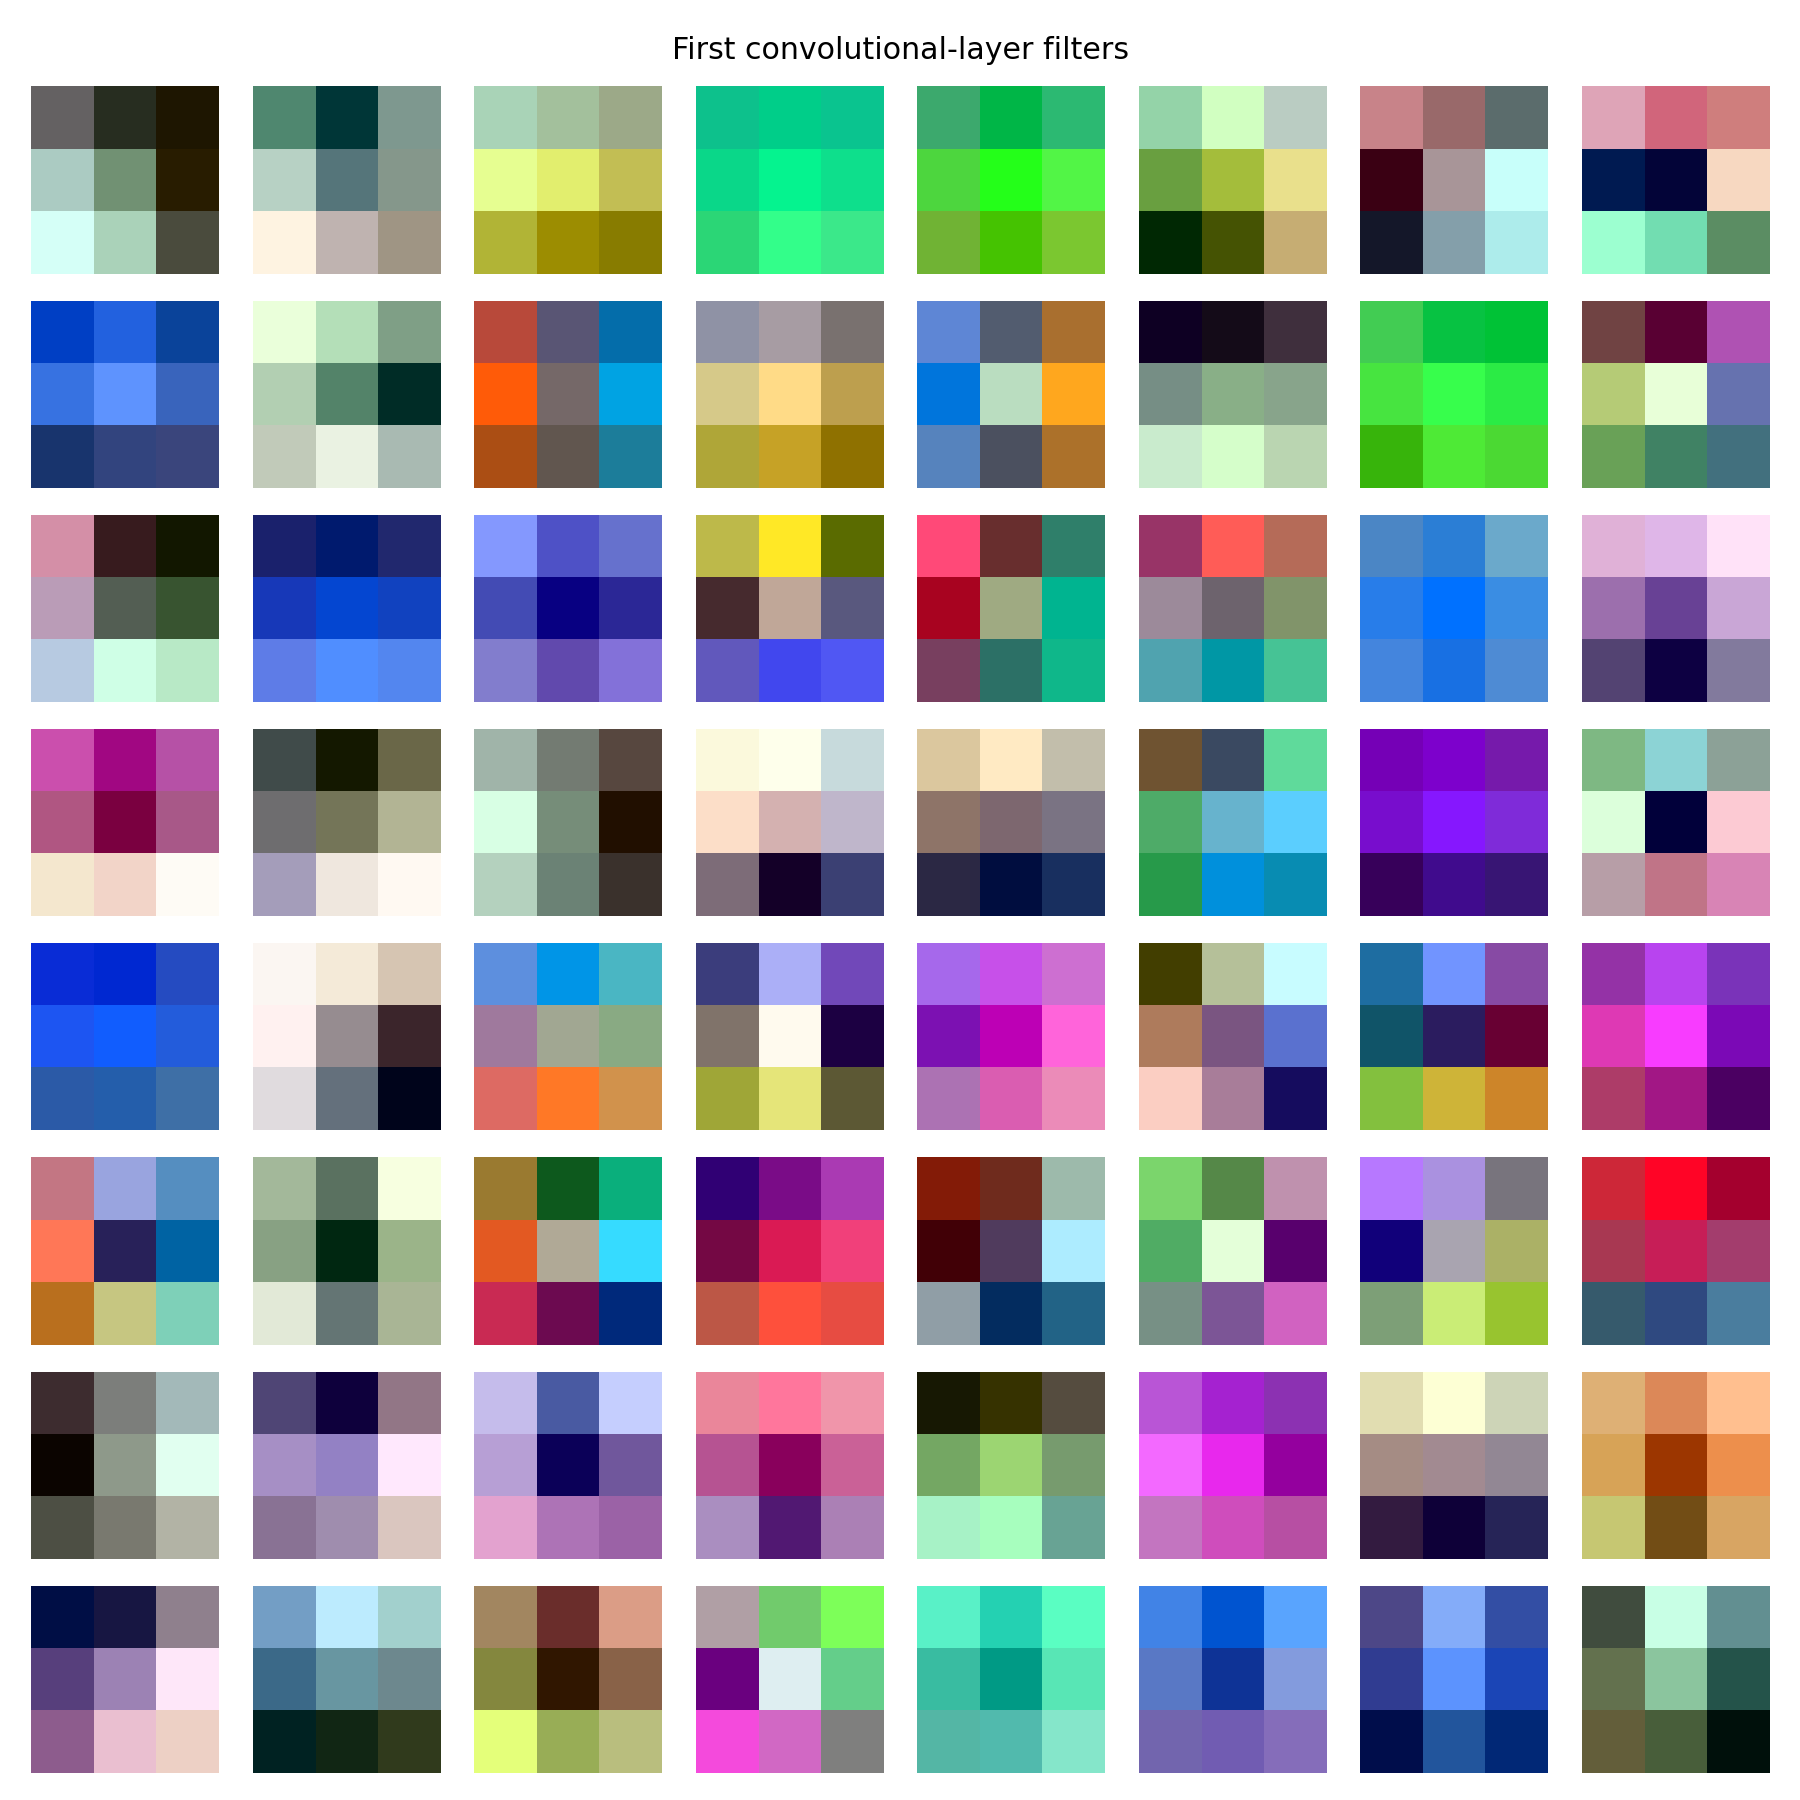
\includegraphics[width=\linewidth]{task1_filters.png}
    \caption{第一层卷积核}
  \end{subfigure}
  \caption{最佳模型的分类行为与低层特征。第一层卷积核学习到了颜色差异、
  方向和局部边缘等模式。}
\end{figure}

逐类准确率中，ship 最高，为 $96.1\%$；cat 最低，为 $81.4\%$，dog 和 bird
也相对较难。这符合低分辨率自然图像中动物类别外观相似、类内变化较大的特点。

\begin{figure}[H]
  \centering
  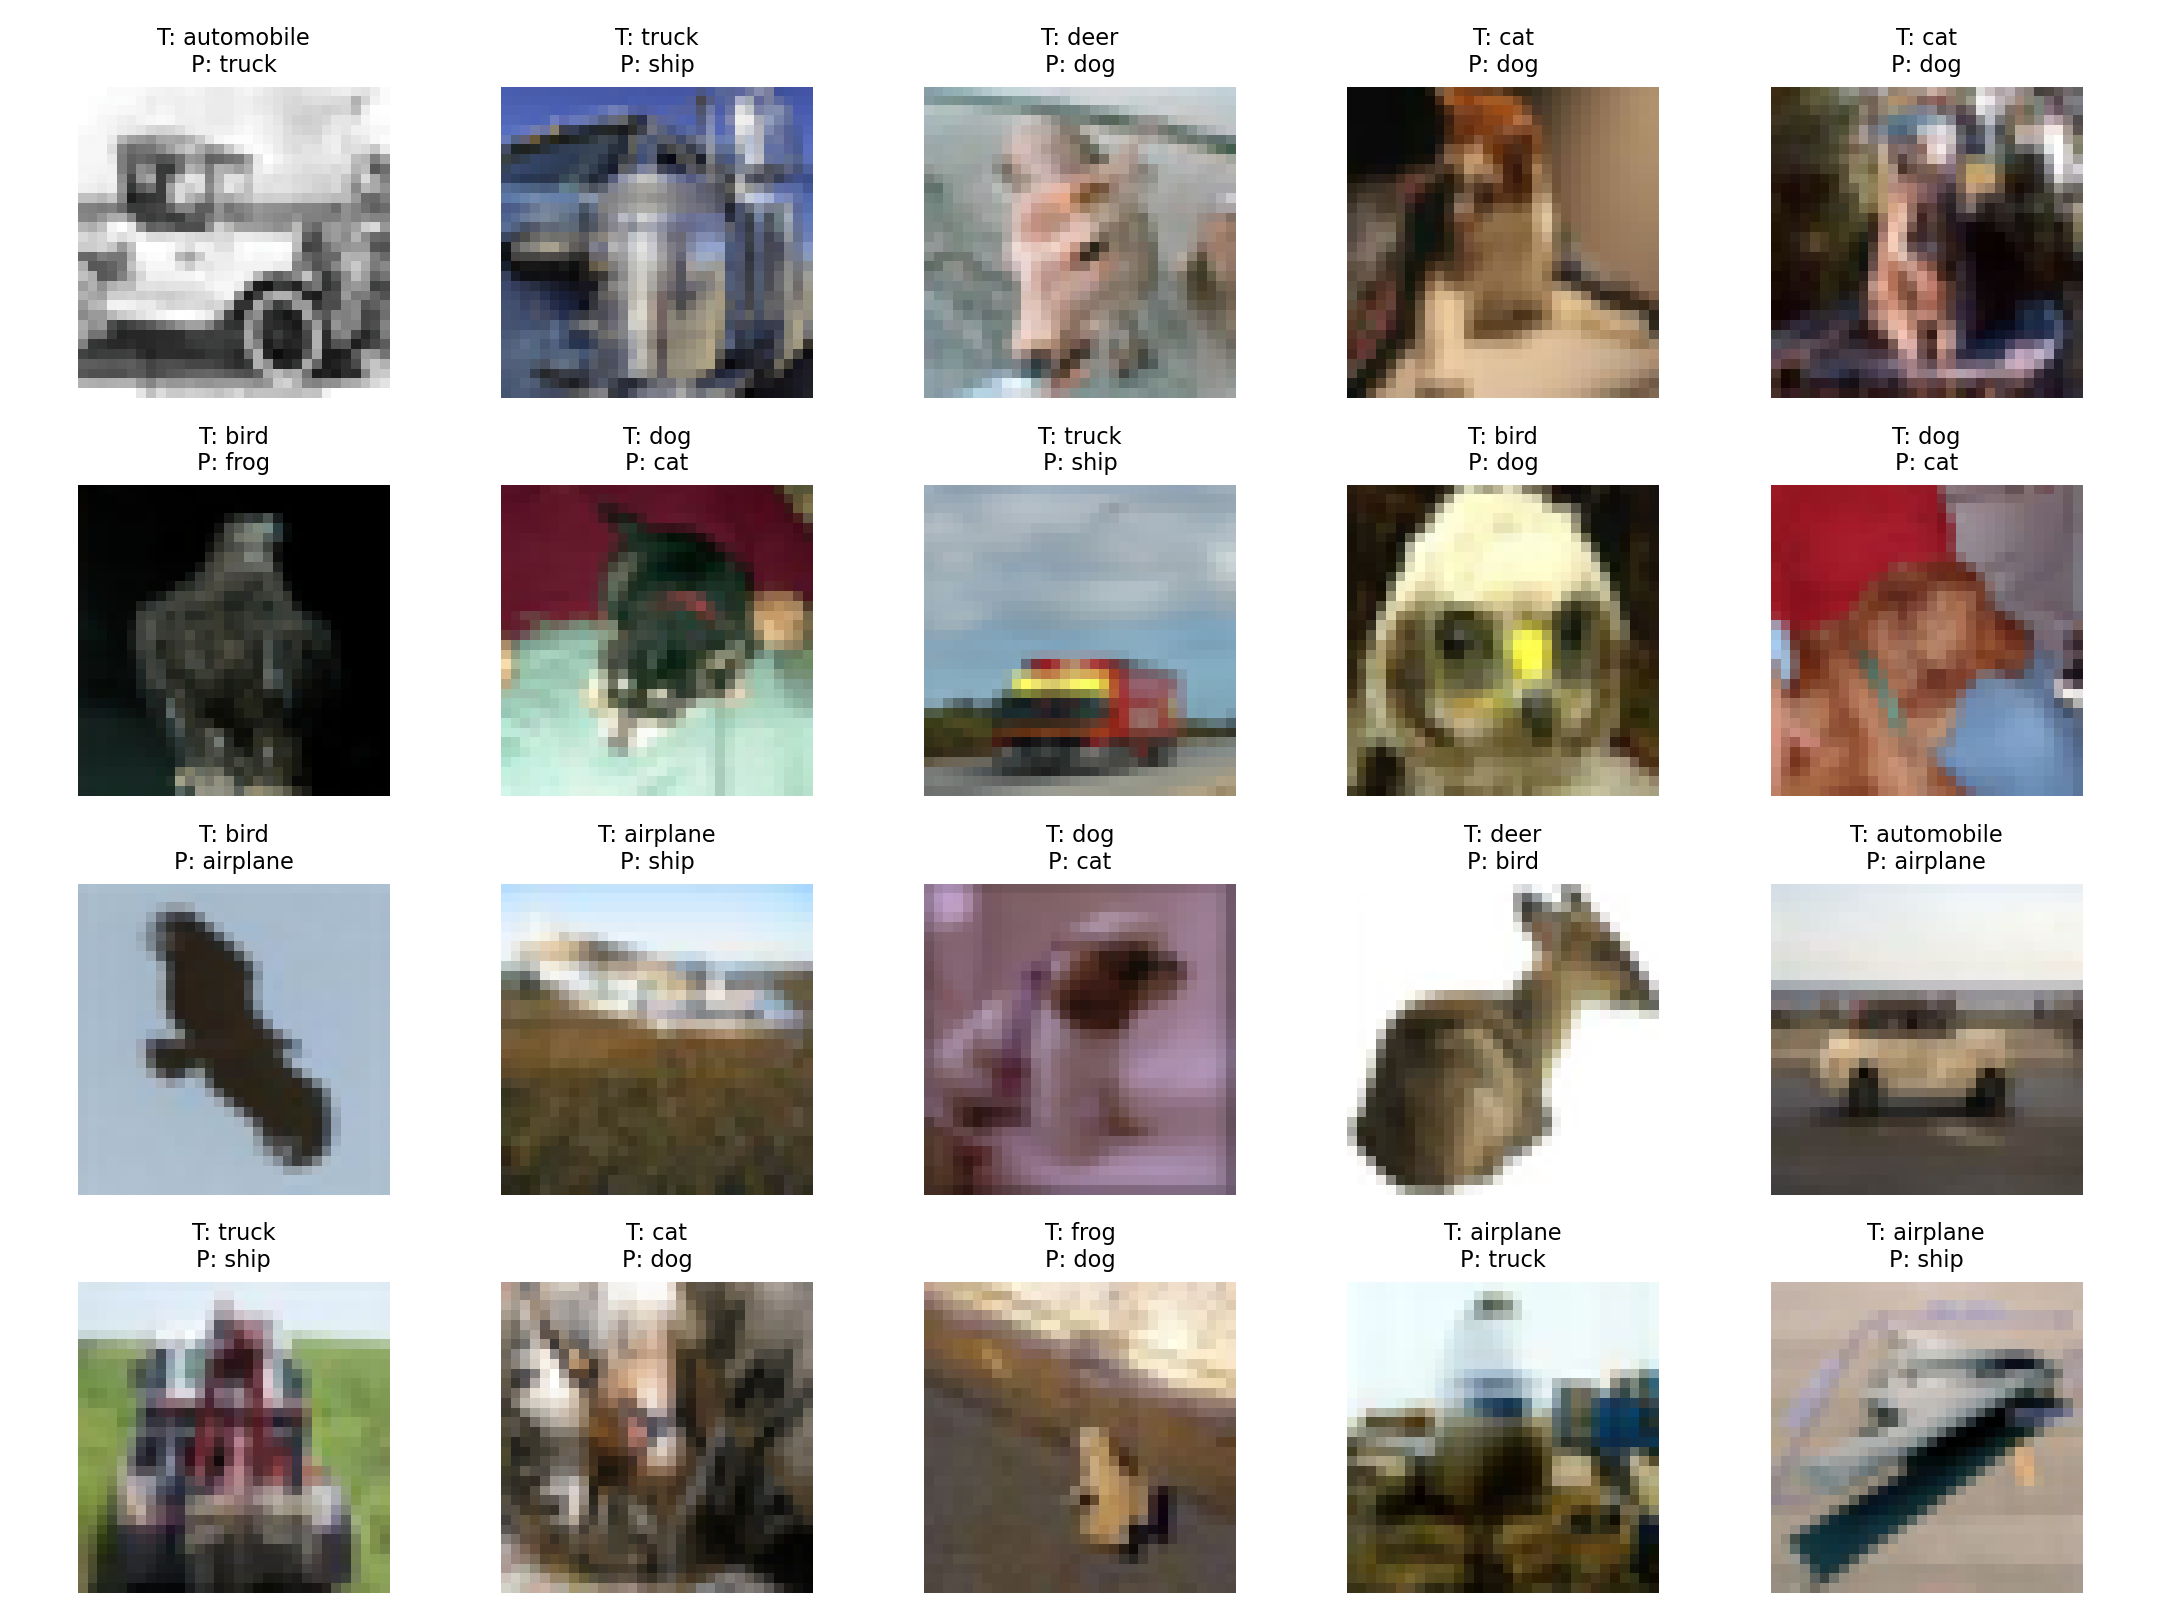
\includegraphics[width=0.9\textwidth]{task1_misclassified.png}
  \caption{最佳模型的部分错误分类样例。错误多出现在视觉特征相近的动物类别，
  或主体较小、背景干扰较强的图像。}
\end{figure}

\section{任务二：Batch Normalization}

\subsection{BN 的原理}

对卷积层某一通道 $c$，设一个 mini-batch 中包含的激活为
$x_{b,c,h,w}$。BN 在 batch 和空间维度上计算均值与方差：
\begin{align}
  \mu_c &=
  \frac{1}{BHW}\sum_{b,h,w}x_{b,c,h,w},\\
  \sigma_c^2 &=
  \frac{1}{BHW}\sum_{b,h,w}(x_{b,c,h,w}-\mu_c)^2.
\end{align}
归一化及可学习仿射变换为
\begin{align}
  \hat{x}_{b,c,h,w}
  &=\frac{x_{b,c,h,w}-\mu_c}{\sqrt{\sigma_c^2+\epsilon}},\\
  y_{b,c,h,w}&=\gamma_c\hat{x}_{b,c,h,w}+\beta_c.
\end{align}
其中 $\epsilon$ 用于数值稳定，$\gamma_c$ 和 $\beta_c$ 为可学习参数。
训练时使用当前 mini-batch 统计量并维护 running mean/variance；测试时使用
训练期间累积的 running statistics，保证预测不依赖测试 batch 的组成。

\subsection{BN 对优化的作用}

BN 最初被解释为减轻 ``internal covariate shift'' \cite{batchnorm}。后续研究
指出，BN 还会改变网络的参数化与优化几何，使局部一阶近似更可靠
\cite{santurkar2018}。归一化能够稳定各层激活尺度，改善深层网络中的梯度
传播，降低训练初期的数值不稳定性，并使模型更快进入低 loss 区域。mini-batch
统计量引入的随机性还具有一定正则化效果。

\subsection{VGG-A 有无 BN 的比较}

VGG-A 使用五个卷积阶段，通道数为 $(64,128,256,512,512)$，每阶段后进行
最大池化；分类器使用三层全连接层。BN 版本仅在每个卷积层之后、ReLU 之前
加入 BatchNorm2d，其余结构、数据划分、随机种子、优化器和学习率均相同。

实验使用完整的 45,000 张训练图像、5,000 张验证图像和 10,000 张测试图像。
优化器为 Adam，学习率为 $10^{-3}$，batch size 为 128，共训练 20 epoch。
为隔离 BN 的影响，该实验不使用数据增强。

\begin{table}[H]
  \centering
  \caption{VGG-A 有无 BN 的比较}
  \begin{tabular}{lrrrr}
    \toprule
    模型 & 参数量 & 最佳验证准确率 & 测试准确率 & 最佳 epoch \\
    \midrule
    VGG-A & 9,750,922 & 75.24\% & 75.88\% & 17 \\
    VGG-A + BN & 9,753,674 & 82.88\% & 82.50\% & 12 \\
    \bottomrule
  \end{tabular}
\end{table}

BN 仅增加 2,752 个可学习参数，却将测试准确率提高 6.62 个百分点；同时，
BN 模型在第 12 epoch 达到最佳验证结果，而无 BN 模型到第 17 epoch 才达到
最佳结果，进一步体现了 BN 的收敛速度优势。

\begin{figure}[H]
  \centering
  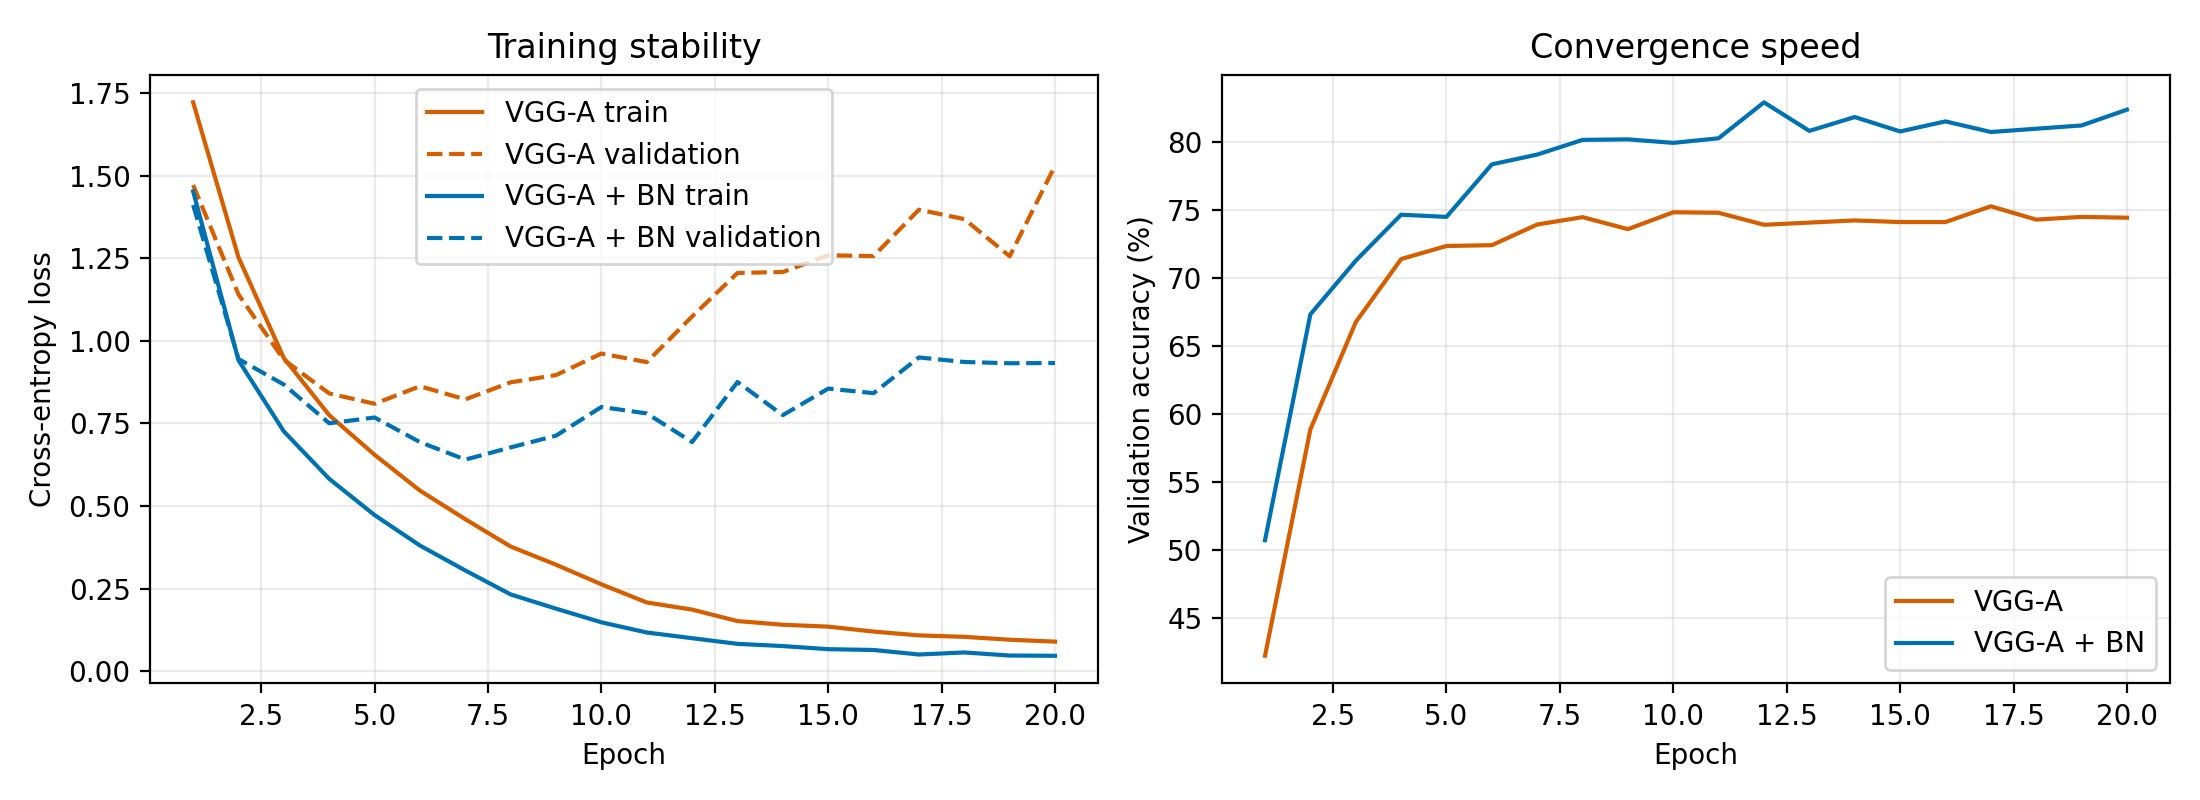
\includegraphics[width=\textwidth]{task2_bn_comparison.png}
  \caption{VGG-A 有无 BN 的训练比较。BN 模型在前几个 epoch 就获得明显更高
  的验证准确率，并在大部分训练阶段保持更低的 loss。}
\end{figure}

\subsection{Loss landscape}

按照项目给出的简化方法，分别使用学习率
\[
  \{10^{-4},5\times10^{-4},10^{-3},2\times10^{-3}\}
\]
训练模型，并记录每个优化 step 的 loss。对于同一个 step $t$，定义
\begin{align}
  L_{\min}(t)&=\min_{\eta} L_{\eta}(t),\\
  L_{\max}(t)&=\max_{\eta} L_{\eta}(t),\\
  R(t)&=L_{\max}(t)-L_{\min}(t).
\end{align}
图中的阴影区域位于 $L_{\min}$ 和 $L_{\max}$ 之间，$R(t)$ 表示模型在不同
学习率下的 loss 变化范围。较大的 $R(t)$ 表明训练对学习率更敏感。

\begin{figure}[H]
  \centering
  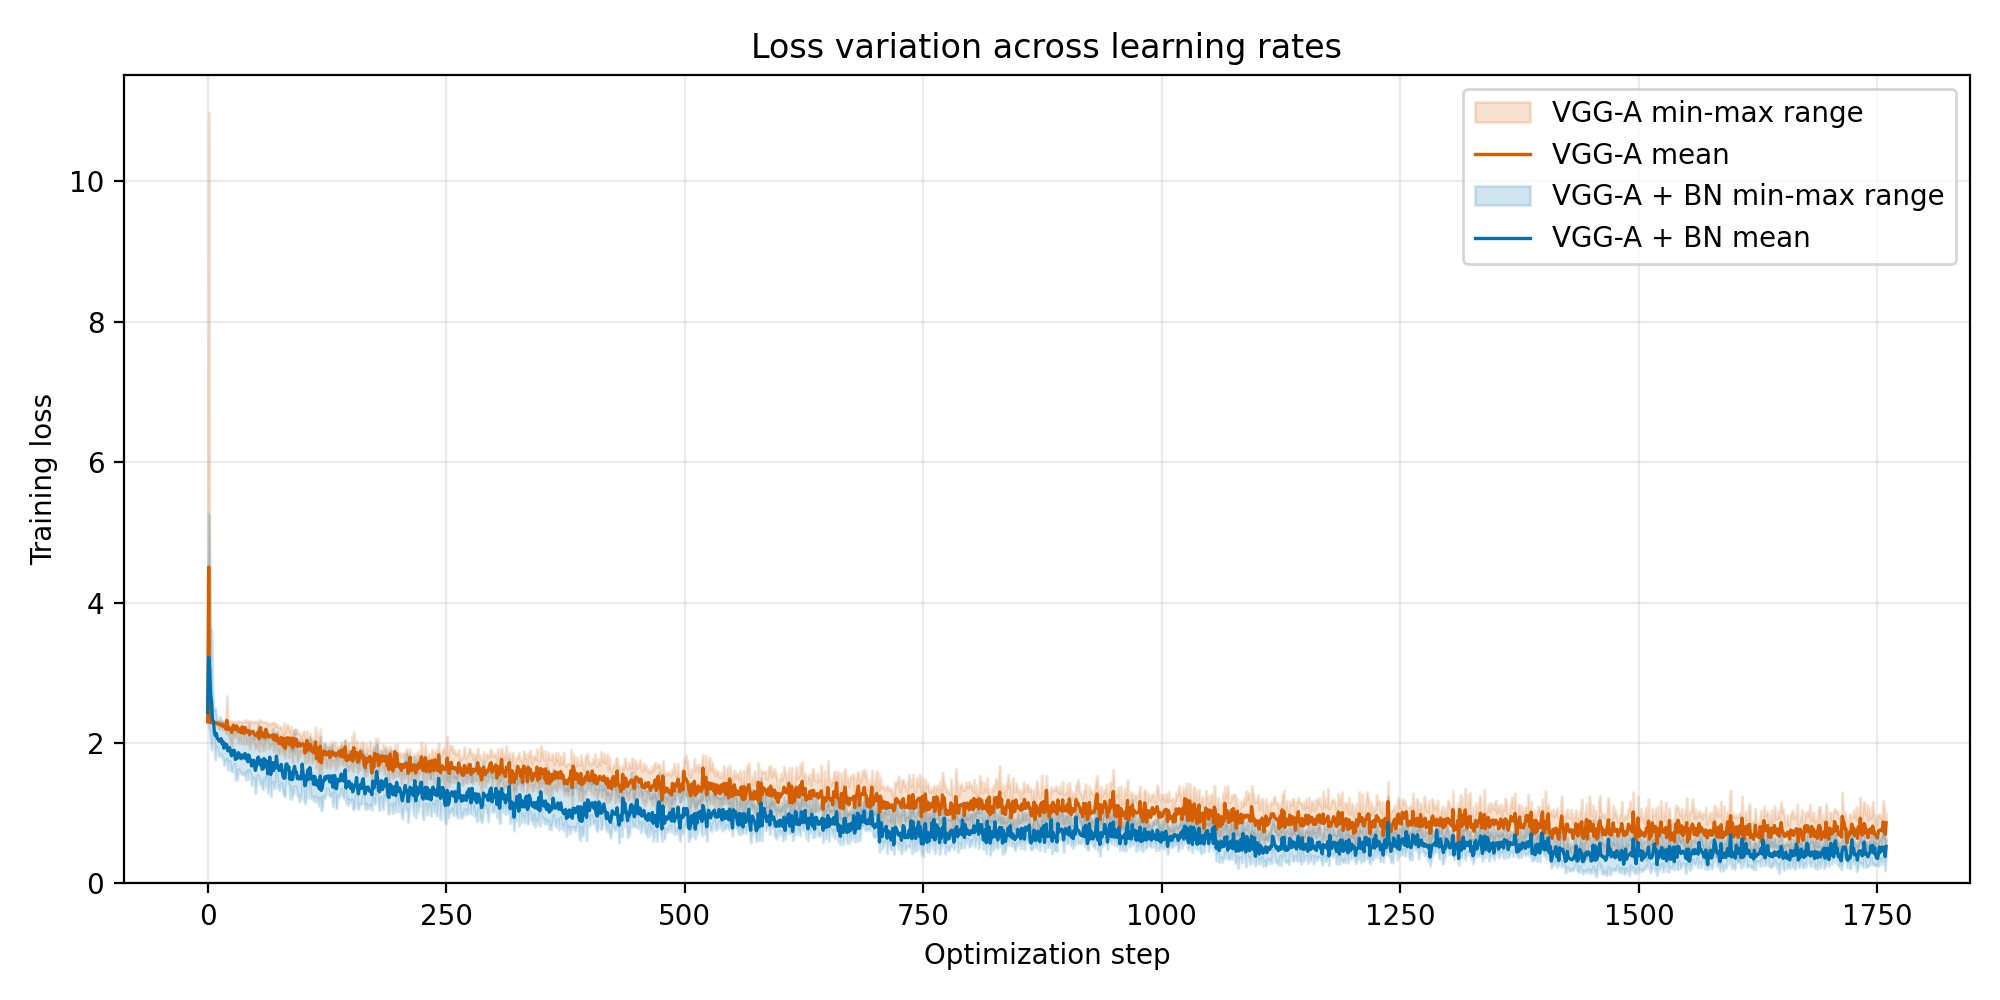
\includegraphics[width=\textwidth]{task2_landscape.png}
  \caption{四个学习率下的 loss min--max 区间。无 BN 模型在训练初期产生了
  明显的极端 loss 峰值。}
\end{figure}

无 BN 模型的最大跨度为 8.67，BN 模型为 3.01，说明 BN 显著降低了训练初期
最坏情况下的学习率敏感性。BN 模型在大部分优化步中还具有更低的平均 loss。

\begin{figure}[H]
  \centering
  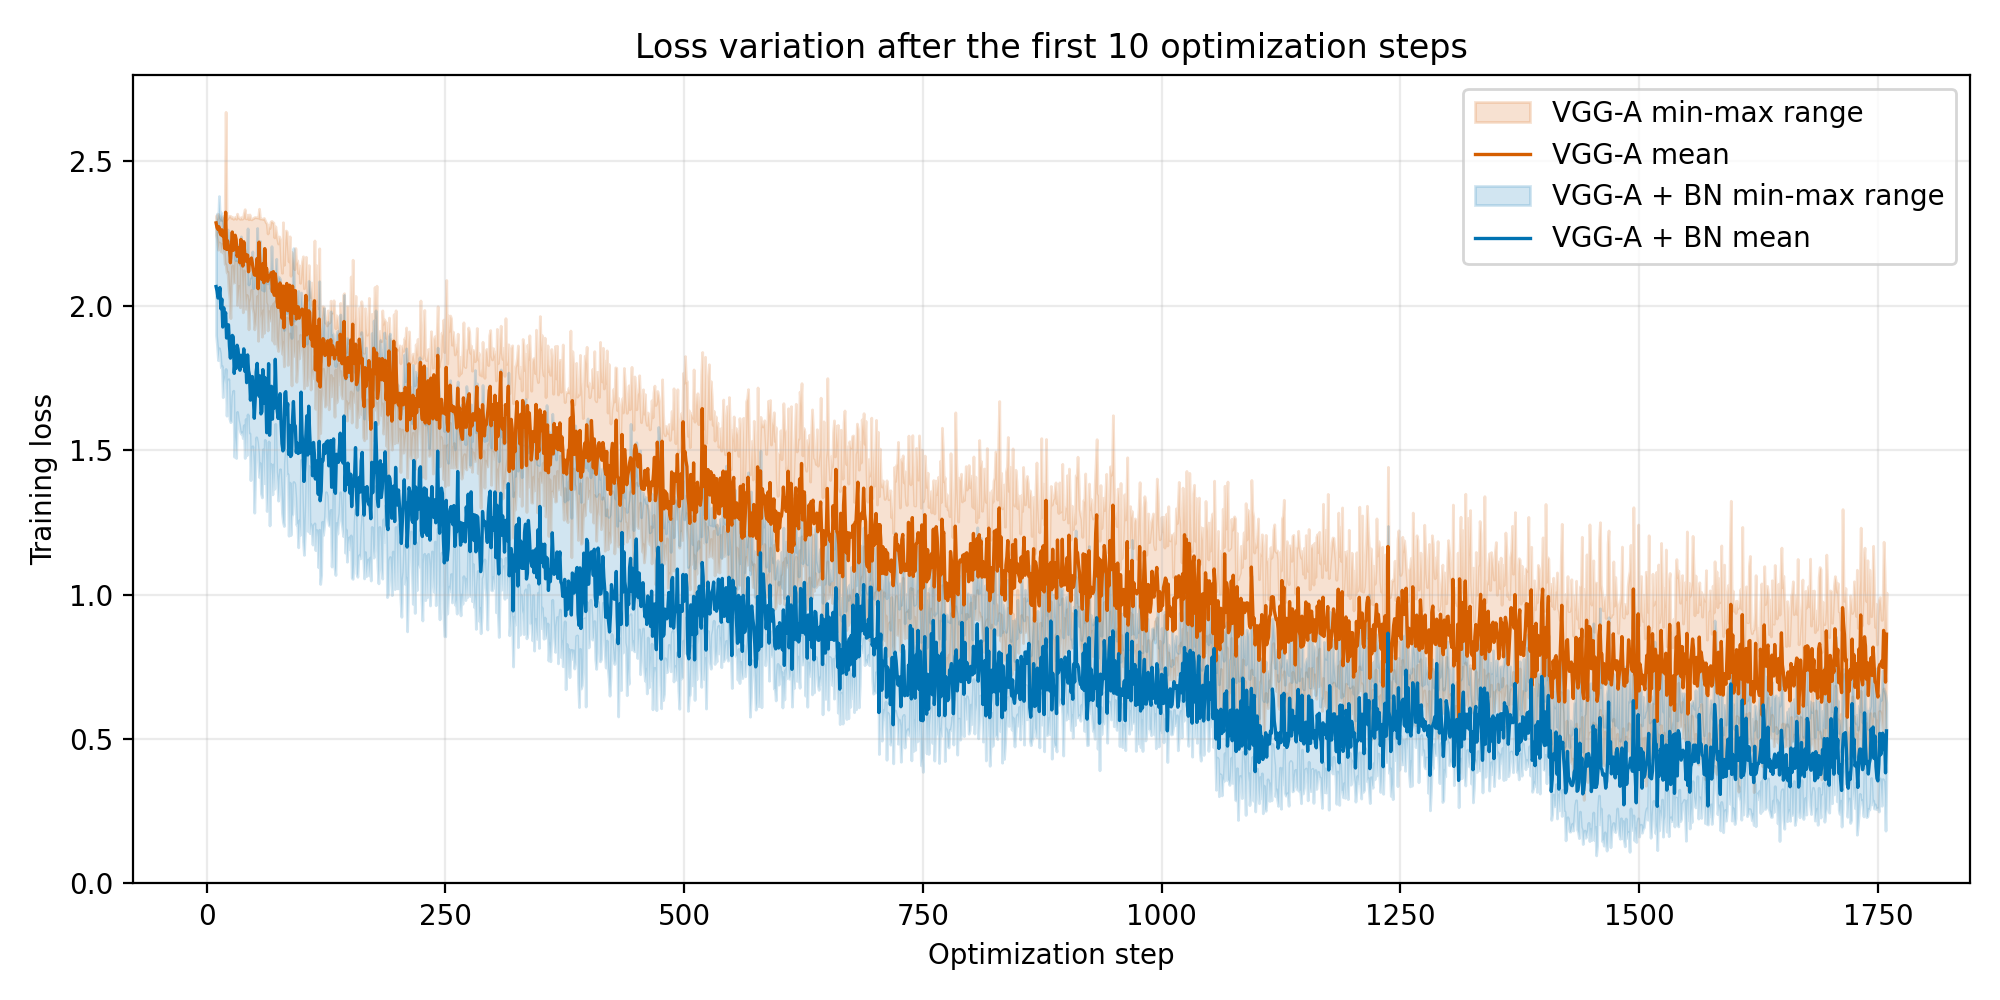
\includegraphics[width=\textwidth]{task2_landscape_zoomed.png}
  \caption{去掉前 10 个优化 step 后的放大图。BN 的平均 loss 更低，但
  min--max 区间并非始终更窄。}
\end{figure}

去除前 10 个 step 后，两者的平均跨度几乎相同：BN 为 0.444，无 BN 为
0.443；对应最大跨度分别为 0.923 和 0.755。结合平均 loss 曲线可知，BN 的
主要优势体现在降低训练初期的极端波动，并使模型更快进入较低 loss 区域。

\subsection{梯度可预测性与局部变化}

为补充分析优化过程，记录最后一层分类器权重的梯度 $\bm{g}_t$，计算连续梯度
余弦相似度
\[
  P_t = \frac{\bm{g}_t^\top \bm{g}_{t-1}}
  {\|\bm{g}_t\|_2\|\bm{g}_{t-1}\|_2},
\]
以及梯度变化与参数移动距离之比
\[
  D_t = \frac{\|\bm{g}_t-\bm{g}_{t-1}\|_2}
  {\|\bm{w}_t-\bm{w}_{t-1}\|_2}.
\]
较高的 $P_t$ 表示连续梯度方向更一致；较低的 $D_t$ 通常可解释为局部梯度
变化更缓慢。

\begin{figure}[H]
  \centering
  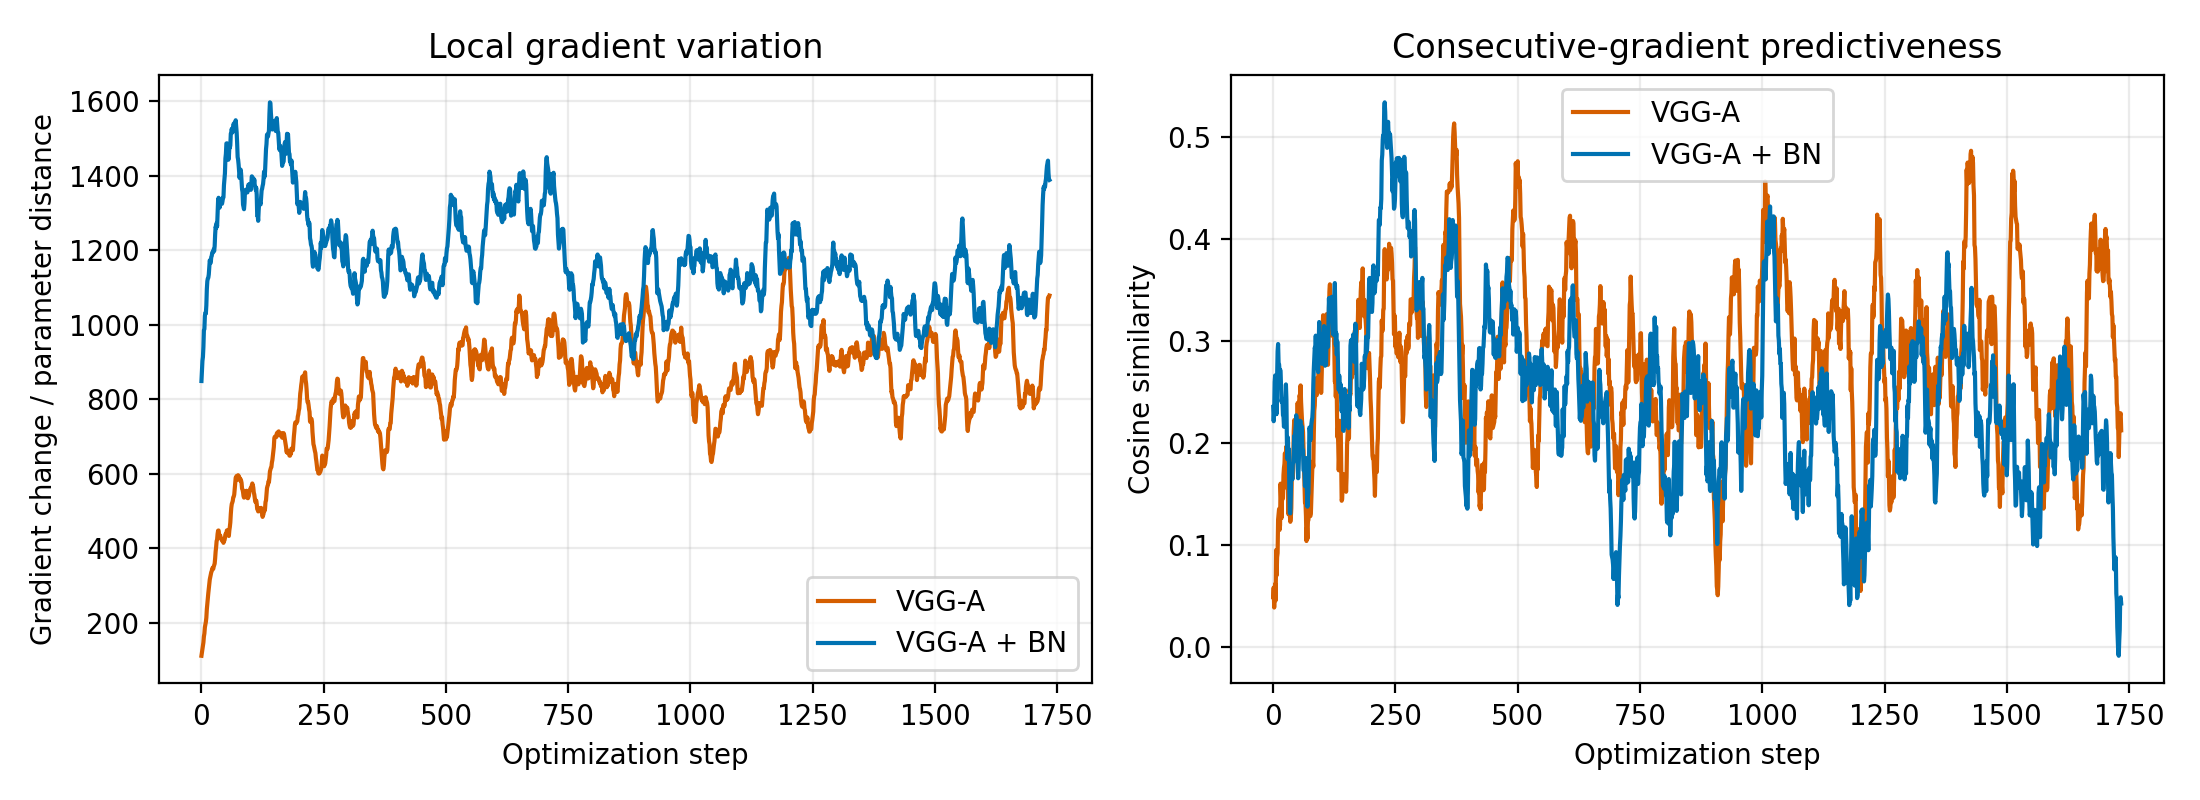
\includegraphics[width=\textwidth]{task2_gradient.png}
  \caption{局部梯度变化与连续梯度方向可预测性。}
\end{figure}

BN 的平均连续梯度余弦相似度为 0.225，无 BN 为 0.260；$D_t$ 的中位数分别
为 152.73 和 87.67。该简化测量未观察到 BN 在这两个指标上的改善。可能原因
包括仅观察最后一层梯度、mini-batch 噪声及参数尺度差异。因此，本文主要依据
分类性能、收敛速度和训练初期的 loss 稳定性评价 BN 的优化效果。

\section{结论}

任务一完成了网络结构、通道数、损失函数、正则化、激活函数和优化器的系统
比较。最终采用 SGD 的定制 CNN 在 CIFAR-10 上达到 $92.06\%$ 测试准确率，
参数量约 115 万。混淆矩阵、卷积核和错误样例进一步揭示了模型在不同类别上的
行为。

任务二实现并比较了 VGG-A 与 VGG-A + BN。全量数据上的受控实验表明，BN
用极少的新增参数换来了明显更快的收敛和 6.62 个百分点的测试准确率提升。
多学习率实验
表明 BN 显著缓解训练初期的极端 loss 波动，并使平均优化轨迹进入更低 loss
区域。简化的梯度方向和局部变化指标没有呈现改善。总体而言，实验支持 BN
能改善深层网络的优化条件和训练效率，同时也说明其作用不能被简单概括为
“所有波动指标都变小”。

\begin{thebibliography}{9}

\bibitem{cifar10}
A. Krizhevsky and G. Hinton,
\newblock ``Learning Multiple Layers of Features from Tiny Images,''
\newblock Technical Report, University of Toronto, 2009.

\bibitem{batchnorm}
S. Ioffe and C. Szegedy,
\newblock ``Batch Normalization: Accelerating Deep Network Training by
Reducing Internal Covariate Shift,''
\newblock in \emph{Proceedings of ICML}, 2015.

\bibitem{santurkar2018}
S. Santurkar, D. Tsipras, A. Ilyas, and A. Madry,
\newblock ``How Does Batch Normalization Help Optimization?''
\newblock in \emph{Advances in Neural Information Processing Systems},
2018.

\bibitem{adam}
D. P. Kingma and J. Ba,
\newblock ``Adam: A Method for Stochastic Optimization,''
\newblock in \emph{Proceedings of ICLR}, 2015.

\end{thebibliography}

\end{document}
